\chapter{How to Write a Novel: 私が実証してきた 12-step process}

この講義には黒板上の derivation はない。だが、それに構造的によく似たものは含まれている。Jenkins は、novel を書くことに対する beginner の diffuse な fear を、constraints、tests、update rules の sequence へ変えていく。順序が重要である。まず object を define し、ついで project を choose し、それをどのように carry するのか、どのように see されるべきか、どのように begin しなければならないか、そして maximum pressure の point へ向けてどのように drive され、そののち resolve されねばならないかを decide するのである。

\begin{remark}
この章の displayed formulas は、lecture の procedural logic を cautious に reconstruct したものである。on-screen notation の transcription ではない。advice の structure を explicit にしているにすぎない。
\end{remark}

\section{fear から method へ}

Jenkins は、ground を clearing することから始める。process の前に、craft の前に、motivation の前に、彼は何が discussion の object なのかを tell する。present lecture において、novel は fiction である。これは elementary に sound するが、正しい第一歩である。target を fix し、talk が writing in general の looser な discussion へ dissolve してしまうのを防ぐからだ。

\begin{definition}
この講義の意味において、novel とは fiction の work である。
\end{definition}

\begin{equation}
\text{novel}=\text{fiction}.
\end{equation}

そこから lecture は、real obstacle へ向けて at once に pivot する。listener には idea があり、write したいと思っており、ひょっとすると words の gift があると even told されているかもしれない。だが privately には、whole novel は finish するには too large であるか、finish するにしても well に finish するには too difficult なのではないかという fear がある。Jenkins は、その fear に vague な inspiration への appeal で answer しない。repeatable な process を promise することによって answer するのである。

彼はまた、preserve すべき二つの motivational beats を insert する。第一に、practiced な novelist でさえ、自分の idea が book を carry できるのか、writing が十分 good になるのかを continue to worry している。第二に、revision の bonus step と、submission の前に every word を check するための checklist があるので、lecture の end まで stay してほしいと彼は listener に ask する。すでに lecture は、自分が recommend することを自ら doing しているのである。problem を establish し、structure を promise し、payoff を setup しているのだ。

\subsection{Question \& Answer}

\paragraph{Question.} whole novel を書くに enough なものが自分にあるのか fear しているなら、どう proceed すればよいのか。

\paragraph{Answer.} fear が vanish するのを wait しない。indefinite な ambition を、concrete な steps の sequence へ置き換えるのである。Jenkins の最初の promise は、writing が easy になるということではない。それが intelligible になり、repeatable になりうるということだ。

\section{story を choose することと middle を survive すること}

第一の substantive question は selection である。私たちには many story ideas があるかもしれない。Jenkins は、それを solution ではなく initial condition として treat する。problem は、book を carry するに enough な weight を持ち、first pages の excitement が worn off したあとでも work に戻ってこさせるに enough な emotional force を持つ one idea を choose することにある。

彼はすぐに practical な scale を give する。winning idea は、merely clever な opening や scene や premise ではなく、substantial length の novel を carry できなければならない。structurally には、novel はまず三つの regions に partition される。

\begin{equation}
\text{Opener} \to \text{Middle} \to \text{Ending}.
\end{equation}

lecture の初期 section でもっとも memorable な phrase は、この difficult な region に name を与えるものである。

\begin{definition}
marathon of the middle とは、opener と ending の between にある、novel の long central stretch のことであり、そこでは drama、tension、conflict、action、そして payoffs を demand する setups が sustained されなければならない。
\end{definition}

ここで Jenkins は、``write what you love'' という usual な advice より exact になる。idea が beginning で spark するだけでは enough ではない。それは duration を survive できなければならない。idea が tested されるのは、その novelty によって alone ではなく、opening の energy が fade したあと、ending が still in sight でないその interval において、それでもなお私たちを draw back し続けるかどうかによってである。

lecture はそのあと、remarkably useful な response test を与える。Jenkins は writer 自身の reaction を、page 上の story の energy に関する local detector として treat する。

\begin{align}
\text{if it bores us} &\Rightarrow \text{it puts the reader to sleep},\\
\text{if it feels flat} &\Rightarrow \text{we lose the reader},\\
\text{if it chokes us up} &\Rightarrow \text{the reader sobs},\\
\text{if it makes us smile} &\Rightarrow \text{the reader is warmed}.
\end{align}

これは mere な sentiment ではない。operational rule である。writer 自身の felt response は、narrative が still carrying force しているかどうかについての evidence なのだ、と Jenkins は言っているのである。

\subsection{Question \& Answer}

\paragraph{Question.} どの story idea が actual に novel を carry できるのか、どうすれば分かるのか。

\paragraph{Answer.} endurance に against して idea を test するのである。winning idea とは、middle を survive する one であり、work が repetitive で difficult で discouraging になったときでも、それでも keyboard へ pull してくる one なのだ。

\paragraph{A worked filter.} lecture の selection rule は、short な update procedure として stated できる。

\begin{enumerate}
\item candidate ideas の set から start する。
\item どれが still 私たちを work へ draw back してくるかを ask する。
\item strong な opening image に against ではなく、middle に against してその idea を test する。
\item frustration と repetition の under でも durable に remain する passion をもつ idea を keep する。
\end{enumerate}

\section{temperament、structure、そして classical sequence}

project が chosen されると、lecture は次に、それにどう work するのかを問う。Jenkins は familiar な distinction、outliner と pantser を introduce する。outliner は architecture が in advance に laid out されていることを want する。pantser は seed から begin し、writing しながら path を discover する。彼は second temperament の best-known example として Stephen King を invoke する。

だが lecture は、これを tribal argument に let しない。Jenkins は explicitly に false opposition を dissolve する。neither method が intrinsically better なのではない。many writers は hybrids であり、some map の security と discovery の freedom の both を want する。彼自身は strongly に pantser side へ identify しているが、それでもなお、自分が何を doing しているのかについて some idea なしに never start しないのだと immediately add する。この qualification が crucial である。これが私たちを、talk の first real formal model へ carry していくからである。

\subsection{Question \& Answer}

\paragraph{Question.} 必ず outline しなければならないのか。それとも、go しながら story を discover してもよいのか。

\paragraph{Answer.} go しながら much を discover してもよい。だが discovery は structure を abolish しない。temperament が何であれ、novel には still、opening pages のあとで work が stall してしまうのを prevent するに enough robust な carrying sequence が必要なのである。

Jenkins はそこから Dean Koontz の ``classic story structure'' を cite する。これが lecture の clearest algorithmic backbone であり、私たちはそれを compact な symbolic form で preserve すべきである。

\begin{equation}
T_0 \to T_1 \to T_2 \to T_3,
\end{equation}
where
\begin{align}
T_0&=\text{terrible trouble introduced early},\\
T_1&=\text{progressively worsening trouble},\\
T_2&=\text{the predicament appears hopeless},\\
T_3&=\text{the hero wins through developed strength and insight}.
\end{align}

\begin{figure}
\centering
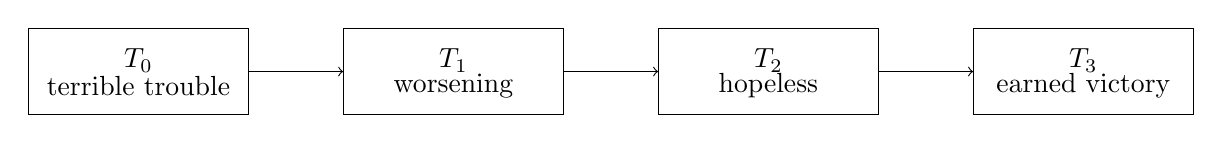
\begin{tikzpicture}
\draw (-1.4,0.55) rectangle (1.4,-0.55);
\node at (0,0.14) {$T_0$};
\node at (0,-0.18) {terrible trouble};

\draw (2.6,0.55) rectangle (5.4,-0.55);
\node at (4.0,0.14) {$T_1$};
\node at (4.0,-0.18) {worsening};

\draw (6.6,0.55) rectangle (9.4,-0.55);
\node at (8.0,0.14) {$T_2$};
\node at (8.0,-0.18) {hopeless};

\draw (10.6,0.55) rectangle (13.4,-0.55);
\node at (12.0,0.14) {$T_3$};
\node at (12.0,-0.18) {earned victory};

\draw[->] (1.4,0) -- (2.6,0);
\draw[->] (5.4,0) -- (6.6,0);
\draw[->] (9.4,0) -- (10.6,0);
\end{tikzpicture}
\end{figure}

この schematic figure は、video からの visual evidence ではない。Jenkins が words で述べる sequence の cleaned reconstruction である。それが私たちに tell すべきなのは、lecture が必要としていることそのものである。narrative pressure は random ではない。それは early に trouble を introduce し、それを step by step に worsen し、premature な relief を refuse し、transformed protagonist を through した resolution においてのみそれを resolve するように built されるのだ。

Jenkins は、この structural passage を strong な imperative で close し、次の steps を prepare する。whatever basic form を use するにしても、私たちは beginning から readers の throat を grab し、never let go してはならない、と。character へ move するのは、その after である。

\section{character、research、そして point of view}

lecture はいま、engine から carrier へ pass する。characters がその pressure を bear できなければ、plot structure は by itself では empty である。Jenkins の first demand は、protagonist が arc を持つことだ。end までには、lead は different な、preferably better な person になっていなければならない。したがって later の victory は arbitrary な success ではありえない。それは development から arise しなければならないのだ。

second condition が immediately follow する。protagonist には flaws があるべきだ。だがその flaws が、reader を outset から push away してしまうほど repulsive であってはならない。opposing side では、antagonist は formidable で compelling でなければならない。Jenkins は、ここでの beginner's mistake を very clearly に述べる。villain は、story の slot が villain を require するという merely その理由で evil なのではない。most villains は、自分が right だと思っている。したがって antagonist にも、intelligible な motives が必要なのである。

same principle は outward に extend する。important な orbital characters は、central casting から来た stock figures 以上のものでなければならない。Jenkins は、それらを develop するための longer な question list に mention する。だが transcript は precisely その point で corrupted する。したがって私たちは、stable なものだけを preserve すべきである。names は distinct であるべきであり、initials は blur together してはならず、characters は、reader がそれらを confuse しない enough に、look も sound も different であるべきだ。

この point で lecture は、useful な coupled variables の pair を introduce する。lead character は outward な problem に face している。だが inward な turmoil によって alive になる。external goal と internal weakness は separated されてはならない。story は、それらを together に drive することによって work するのだ。

research が next に enter する。そしてここで lecture は concrete である。fiction は invented である。だがそれでも believable でなければならない。fantasy や science fiction でさえ、reader が disbelief を suspend するためには internally に hold together していなければならない。Jenkins は preserve しておく価値のある compact ratio を give する。

\begin{equation}
\text{Research}=\text{flavor},\qquad \text{Story}=\text{main course}.
\end{equation}

それから彼は、working novelist が actual に use しうる resources の kinds を name する。

\begin{itemize}
\item atlases と world almanacs,
\item encyclopedias と search engines,
\item interviews, in person or by call,
\item さらには YouTube や thesauri のような ordinary な tools.
\end{itemize}

point は glamour ではない。geographical、cultural、technological な details を、reader が story から fall out しない enough に right にすることにある。Jenkins はまた、important な caveat を add する。futuristic fiction では、私たちは many technical details を invent することになる。だが invented systems であっても、それは make sense し、consistent に remain しなければならないのだ。

research から lecture は naturally に point of view へ move する。これは、Jenkins が insist するように、first、second、third person の among の grammatical choice では merely ない。story の camera として誰が function するのかを decide することなのである。\(s\) を scene、\(\mathrm{POV}(s)\) をその perspective character としよう。すると lecture の operative restriction は

\begin{equation}
|\mathrm{POV}(s)|=1.
\end{equation}
と stated できる。

Jenkins は prose でこの rule を state する。one perspective character per scene であり、彼自身は one per chapter を prefer し、ideally には one per novel を prefer すると add する。この bound が set されると、narrative information の channel も also bounded される。

\begin{equation}
\mathrm{Info}(s)=\{\text{see, hear, touch, smell, taste, think}\}_{\mathrm{POV}(s)}.
\end{equation}

again、この notation は ours であって his ではない。だが lecture を faithfully summarize している。narration は、viewpoint character が perceive し、think するものを convey しうるのである。私たちはその mind の中にいて、その character の senses と emotions を use しているのだ。それから Jenkins は、common な beginner's misunderstanding を resolve する。この restriction は、私たちを \emph{not} first person に force するものではない。third person limited は、single perspective channel と fully compatible であり、in fact modern default である。彼が warn しているのは、casual omniscience、つまり一つの scene の inside で multiple heads の in and out を hop する old habit なのである。

\subsection{Question \& Answer}

\paragraph{Question.} point of view は、novel が reveal できるものをどう constrain するのか。

\paragraph{Answer.} point of view は impoverishment ではなく information boundary である。ひとたび scene の perspective character を choose すると、prose は、その character が perceive し、infer し、remember し、think できるものに limited される。それでもなお orbital characters を reveal することはできる。ただし、一度に一つの consciousness の pressure を通してのみである。

\section{things の midst に始まり、reader の mind を trigger する}

step six の just before に、Jenkins は promised していた bonus step at the end を briefly remind する。この reminder は accidental ではない。lecture が style へ turn しているそのあいだも、procedural frame を alive に保っているのだ。それから彼は、next movement を classical term で begin する。\emph{in medias res}、things の midst である。

彼は、predictable な confusion を head off することに careful である。things の midst に begin するとは、necessarily gunfire や chase を mean するわけではない。それは、story が already moving しているべきところで、inert な explanation、scene-setting、background から begin しない、ということを mean する。opening は forward pressure を carry していなければならない。Jenkins はこの rule を characteristic な bluntness で state する。every sentence、いや indeed every word の goal は、reader に next sentence を read させることである、と。

この local law of motion は、

\begin{equation}
\text{sentence } n \Rightarrow \text{desire to read sentence } n+1.
\end{equation}
と書ける。

ついで彼は、opening line の four kinds を classify する。surprise opener、dramatic statement、philosophical opener、poetic opener である。lecture 中で quoted される examples は、literary ornaments としてではなく、different kinds の forward pull の demonstrations として used されている。\(13\) を打つ clock は expectation を violate する。sudden な violence の act は dramatic gap を open する。philosophical generalization は、それを test したい urge を invite する。strange な poetic image は、tone を destabilize し、その image を contain する world への curiosity を stir する。

だが Jenkins は、lecture を first lines で stop させない。strong opener は necessary だが not sufficient である。many novels は energy をもって begin する。だがその直後に explanation へ sink back してしまう。そこで彼は next beat へ push する。reader の mind の theater である。

ここでの claim は、lecture でも strongest なものの一つである。writers として私たちは、scene を reader に exactly our way に see させようとしているのではない。reader 自身の imaginative construction を trigger しようとしているのだ。enough を suggest し、その after は reader の mind が do する。この point で lecture は、telling と showing の famous distinction へ turn する。

\begin{equation}
\text{Telling} \Rightarrow \text{reader is informed},\qquad
\text{Showing} \Rightarrow \text{reader deduces}.
\end{equation}

\subsection{Question \& Answer}

\paragraph{Question.} show rather than tell とは、really どういう意味なのか。

\paragraph{Answer.} それは、abstract な report を、その hidden state を reader が infer できるような concrete evidence に置き換えることを mean する。reader は merely fact を receiving しているのではない。scene を build する helping をしているのである。

\paragraph{A worked update rule.} Jenkins の conversion procedure は、次のように書ける。

\begin{enumerate}
\item abstract report を identify する。tall、angry、cold、frightened、などである。
\item 別の character、あるいは reader が actual に observe できるものは何かを ask する。
\item abstract predicate を、その observable cues に replace する。
\item evidence が by itself meaning を carrying するようになったら、direct report を remove する。
\end{enumerate}

彼の二つの clearest examples は、note form でもよく survive する。

\begin{align}
\text{``He was tall''} &\to \text{others look up at him; he ducks through a doorway},\\
\text{``He was angry''} &\to \text{his face flushes, his throat tightens, his voice rises, his fist hits the table}.
\end{align}

reader は、last step を internally complete する。だから showing は prettier な prose というだけではない。reader に experience の中で a role を与える one way なのである。

\section{escalation、bleakest moment、そして final discipline}

Jenkins が step eight に reach するころには、earlier の structure は concrete form で return する準備ができている。hero は trouble の中へ launched された。ここでの rule は、それぞれの escape attempt が matters を worse にするべきだ、というものである。ここで lecture は、その strongest maxim を与える。

\begin{equation}
\text{Conflict}=\text{engine of fiction}.
\end{equation}

Jenkins は、その point を drive home するために、deliberately over-comfortable な counterexample を offer する。looks、health、money、equipment、happy home、fine office、そして juicy case を持ち込む rich client を兼ね備えた private investigator である。novel が parody でないかぎり、この ease は narrative force を kill する。彼の corrective は brutally simple だ。supports を remove せよ。ease、money、security、equipment、health、domestic stability を take away せよ。protagonist が genuine pressure の under に置かれたとき、story は alive になる。

私たちは escalation rule を、short derivation として restate できる。

\begin{enumerate}
\item real trouble から begin する。
\item each attempted solution によって situation を intensify させる。
\item conveniences を adding するのではなく supports を strip away する。
\item rising pressure を使って、reader を edge of the page に keep する。
\end{enumerate}

そこから lecture は step nine、bleakest moment へ advance する。Jenkins は、story をその own trap からどうやって write out すればよいのか even writer 自身が wonder する point を指す Angela Hunt の phrase を borrow する。lecture の own example は、purposefully に melodramatic である。reformed lover は、now devoted で apparently changed しているのに、wedding の前夜に everything を destroy する。example の point はそこにある。situation は irreparable に look しなければならないのだ。

\begin{definition}
bleakest moment とは、plot の local nadir、つまり protagonist の predicament が writer にとってさえ hopeless に appear する point のことである。
\end{definition}

これによって lecture の late chain が得られる。

\begin{equation}
\text{trouble} \to \text{worsening trouble} \to \text{bleakest moment} \to \text{climax} \to \text{ending}.
\end{equation}

\subsection{Question \& Answer}

\paragraph{Question.} ending が earned に feel される before に、hero の situation はどれほど hopeless に become すべきなのか。

\paragraph{Answer.} easy path out が visible に remain しない enough に hopeless であるべきだ。Jenkins はここで emphatic である。soft escape を invent するな。miracle を inject するな。pressure が uncomfortable になった merely その理由で protagonist に break を与えるな。bleakest moment の whole function は、story が built してきた whatever new muscle and insight を通して action を force することなのだ。

この answer は、lecture がそのあと insist する distinction を prepare する。

\begin{equation}
\text{Climax} \neq \text{Ending}.
\end{equation}

climax は final test であり、confrontation の peak であり、book-length の setups が paid off される point である。ending はその after に来る。quieter ではあるが dispensable ではない。Jenkins は、successful ending の two criteria を give する。それは reader first を置き、reader の investment を honor すること。そして hero を last word まで stage の上に keep することである。つまり、fireworks が over したら simply stop してよいわけではない。still land しなければならないのである。

lecture はそのあと、fictional process から writerly process へ return して close する。bonus step は appendix ではない。whole talk の logic を complete するものなのである。novel が ordered stages を need とするように、それを書く work もそうなのである。Jenkins の final rule は

\begin{equation}
\text{Drafting} \neq \text{Editing}.
\end{equation}
である。

first draft は、inner critic を muted にした状態で written されるべきである。cliches、rough transitions、logical infelicities は、その場で solve することが motion を destroy するなら、その場で solve されるべきではない。revision は later に、separate な mental mode で来る。したがって lecture の final update rule は、次のものである。

\begin{enumerate}
\item perfection のために stopping せずに draft する。
\item drafting pass の during に roughness が remain することを allow する。
\item separate な revision pass で return する。
\item drafting motion が complete してから only、word by word に fine-tune する。
\end{enumerate}

promised された twenty-one-part checklist は、その second mode に belong している。transcript はその contents を preserve していないので、私たちはその role だけを preserve する。それは drafting instrument ではなく、revision instrument なのである。

\section{まとめ}

lecture は fear から始まり、discipline で終わる。その間に、それは large で blurred な ambition を structured progression へ turn する。object を define し、one durable idea を choose し、temperament を structure と distinguish し、story に carrying sequence を与え、pressure を bear できる characters を build し、world を believable にし、prose を coherent な point of view に restrict し、motion の中で begin し、reader が merely receive するのではなく infer するようにし、conflict を increase し、story を its bleakest moment へ drive し、climax を ending と separate し、drafting を editing と separate するのである。

したがって、この chapter の deepest lesson は、writing が formula に reduce できるということではなく、それによって stabilize できるということである。middle を survive できる project を choose し、reader が true に enter できるよう narrative を constrain し、ending が merely arrived at されるのではなく earned されるまで conflict を deepen させるのである。